\newpage

\newcommand{\lonece}[0]{\ensuremath{\ell_1\textup{-CE}}}
\newcommand{\loneerror}[0]{\ensuremath{\mathcal{E}}}
\newcommand{\pluginLoneEst}[0]{\ensuremath{\hat{\mathcal{E}}_{\textup{pl}}}}
\newcommand{\debiasedLoneEst}[0]{\ensuremath{\hat{\mathcal{E}}_{\textup{db}}}}

\section{Additional experiments for section~\ref{sec:verifying_calibration}}
\label{sec:verifying_calibration_appendix_experiments}

\subsection{Debiasing the ECE}
\label{sec:debiasing_ece_experiments}

We propose a way to more accurately estimate the $\ell_1$ calibration error (popularly known as ECE), and run experiments on ImageNet and CIFAR-10 that show that we can estimate the error much better than prior work, which uses the plugin estimator. The key insight is the same as for the $\ell_2$ calibration error---the plugin estimator for the $\ell_1$ calibration error is biased and this bias leads to inaccurate estimates. To estimate the error better we can subtract an approximation of the bias which leads to a better estimate. The main difference is that for the $\ell_1$ calibration error we were not able to approximate the bias with a closed form expression and instead use a Gaussian approximation.

Recall that the $\lonece{}$ is the $\ell_p{}$ calibration error with $p=1$, redefined below:

\begin{definition}
The $\ell_1$ calibration error of $f : \mathcal{X} \to [0, 1]$ is given by:
\begin{align}
\lonece(f) = \expect\big[ \left|f(X) - \expect[Y \mid f(X)] \right| \big]
\end{align}
\end{definition}

Estimating the $\lonece{}$ for many models is challenging (see Section~\ref{sec:challenges-measuring}) so prior work instead selects a binning scheme $\bins{}$ and estimates $\lonece(f_{\bins{}})$ of a model $f$. Suppose we wish to measure the binned calibration error $\loneerror{} = \lonece(f_{\bins{}})$ of a model $f : \mathcal{X} \to [0, 1]$ where $|\bins{}| = B$. Suppose we get an evaluation set $T_n = \{(x_1, y_1), \dots, (x_n, y_n)\}$. Past work typically estimates the $\ell_1$ calibration error using a plugin estimate for each term:

\begin{definition}[Plugin estimator for $\lonece{}$]
  Let $L_k$ denote the data points where the model outputs a prediction in the $k$-th bin of $\bins{}$: $L_k = \{ (x_j, y_j) \in T_n \; | \; f(x_j) \in I_k \}$.
  
  Let $\hat{p}_k$ be the estimated probability of $f$ outputting a prediction in the $k$-th bin:
$\hat{p}_k = \frac{|L_k|}{n}$.

Let $\hat y_k$ be the empirical average of $Y$ in the $k$-th bin: $\hat y_k = \sum_{x, y \in L_k} \frac{y}{|L_k|}$.

Let $\hat s_k$ be the empirical average of the model outputs in the $k$-th bin: $\hat s_k = \sum_{x, y \in L_k} \frac{f(x)}{|L_k|}$.
  
  The plugin estimate for the binned $\ell_1$ calibration error is the weighted squared difference between $\hat y_k$ and $\hat s_k$:
\[ \pluginLoneEst{} = \sum_{k=1}^B \hat{p}_k \lvert \hat s_k - \hat y_k \rvert \]
\end{definition}

The plugin estimate is a biased estimate of the binned calibration error. Intuitively, this is because of the absolute value: on any finite samples $s_k$ and $y_k$ will differ and the absolute value of the difference will be positive, even if the population values are the same. More concretely consider a model $f$ where $\expect[f(X) \mid f(X) \in I_k] = \expect[Y \mid f(X) \in I_k]$ in every bin $k$. In that case the binned calibration error $\loneerror{}$ is $0$. But on any finite samples the plugin estimate $\pluginLoneEst{}$ will be larger than $0$. In particular, the plugin estimator overestimates the binned calibration error, and the extent of overestimation may be different for different models.

To improve the estimate, we can subtract an approximation of the bias. That is, we would like to output $\pluginLoneEst{} - (\expect[\pluginLoneEst{}] - \loneerror{})$ as our estimate of the calibration error, where $\expect[\pluginLoneEst{}] - \loneerror{}$ is the bias. However, $\expect[\pluginLoneEst{}] - \loneerror{}$ is difficult to approximate in closed form. Instead, we propose approximating it by simulating draws from a normal approximation. More precisely, let $y_k = \expect[Y \mid f(X) \in I_k]$. Then, each label in the $k$-th bin is a draw from a Bernoulli distribution with parameter $y_k$. So $\hat y_k$ is the mean of $n \hat p_k$ Bernoulli draws. Assuming that the number of points in each bin is not too small, we can approximate $\hat y_k$ using a Gaussian approximation, and use that to approximate the bias $\expect[\pluginLoneEst{}] - \loneerror{}$.

\begin{definition}[Debiased estimator for $\lonece{}$]
For each $k$, let $R_k$ be a random variable sampled from a normal approximation of the label distribution in the $k$-th bin: $R_k \sim N(\hat y_k, \frac{\hat y_k (1 - \hat y_k)}{n \hat{p}_k})$. The debiased estimate for the binned $\ell_1$ calibration error subtracts an approximation of the bias from the plugin estimate:
\[ \debiasedLoneEst{} = \pluginLoneEst{} - (\expect\Big[\sum_{k=1}^B \hat{p}_k \lvert \hat s_k - R_k \rvert \Big] - \pluginLoneEst{}) \]
\end{definition}

We can approximate the expectation in the debiased estimator by simulating many draws from a normal distribution, which is computationally fairly inexpensive. Note that our proposed estimator is a heuristic approach, and future work should examine whether we can get provably better estimation rates for estimating the $\ell_1$ calibration error, as we did for the $\ell_2$ calibration error. That might involve analyzing our proposed estimator, or may involve coming up with a completely different estimator.

\begin{figure}
  \centering
  \centering
     \begin{subfigure}[b]{0.45\textwidth}
         \centering
         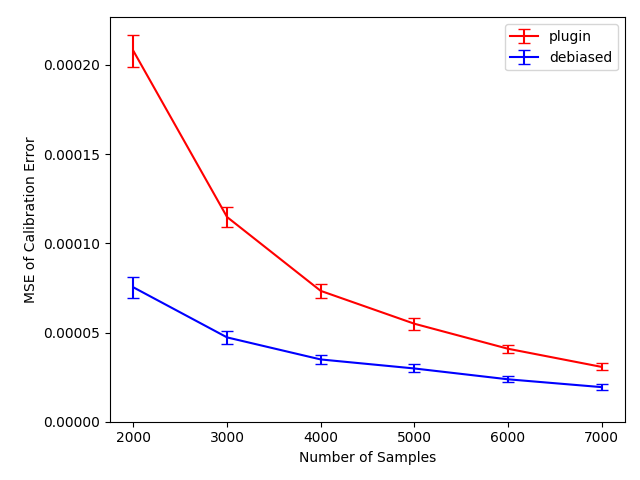
\includegraphics[width=\textwidth]{images/imnet_scaling_ece_curve_15.png}
         \caption{$B = 15$
         }
     \end{subfigure}
     \hfill
     \begin{subfigure}[b]{0.45\textwidth}
         \centering
         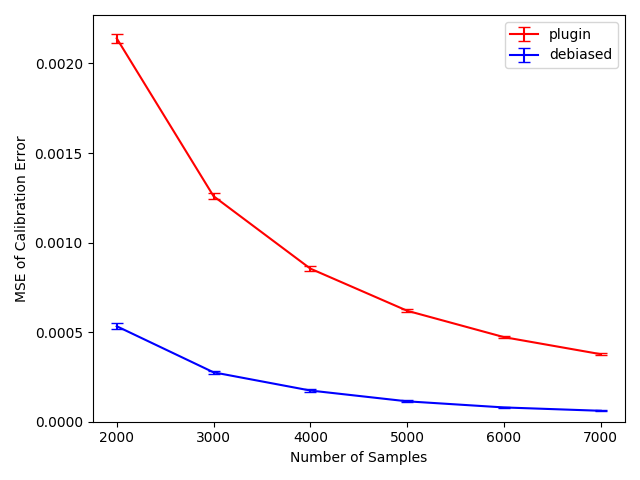
\includegraphics[width=\textwidth]{images/imnet_scaling_ece_curve_100.png}
         \caption{$B = 100$
         }
     \end{subfigure}
  \caption{
    Mean-squared errors of plugin and debiased estimators on a recalibrated VGG16 model on ImageNet with $90\%$ confidence intervals (lower values better). The debiased estimator is closer to the ground truth, which corresponds to $0$ on the vertical axis, and much more so when $B$ is large or $n$ is small.
    Note that this is the MSE of the ECE estimates, not the MSE of the model in Figure~\ref{fig:nan2}.
}
  \label{fig:mse_estimators_imagenet_ece_bins}
\end{figure}

We run multiclass top-label calibration experiment on CIFAR-10 and ImageNet which suggests that the debiased estimator produces better estimates of the calibration error than the plugin estimator. We describe the protocol for ImageNet first, which is similar to the experimental protocol in Section~\ref{sec:verifying_calibration_experiments}. We split the validation set of size 50,000 into two sets $\calset{}$ and $\verifset{}$ of sizes 3,000 and 47,000 respectively. Note that a practitioner would not need so many data points when estimating their model's calibration, we use 47,000 points only so that we can reliably compare the estimators. We use $\calset{}$ to re-calibrate a trained VGG-16 model and select a binning scheme $\bins{}$ so that each bin contains an equal number of points (uniform-mass binning). We calibrate the top probability prediction as described in Section~\ref{sec:formulation} using Platt scaling. For varying values of $n$, we sample $n$ points with replacement from $\verifset{}$, and estimate the binned $\ell_1$ calibration error (ECE) using the plugin estimator and our proposed debiased estimator. We used $B = 100$ or $B = 15$ bins in our experiments. We then compute the squared deviation of these estimates from the binned $\ell_1$ calibration error measured on the entire set $\verifset{}$. We repeat this resampling 1,000 times to get the mean squared deviation of the estimates from the ground truth and 90\% confidence intervals. Figure~\ref{fig:mse_estimators_imagenet_ece_bins} shows that the debiased estimates are much closer to the ground truth than the plugin estimates---the difference is especially significant when the number of samples $n$ is small or the number of bins $B$ is large. Note that having a perfect estimate corresponds to $0$ on the vertical axis.

\begin{figure}
  \centering
  \centering
     \begin{subfigure}[b]{0.45\textwidth}
         \centering
         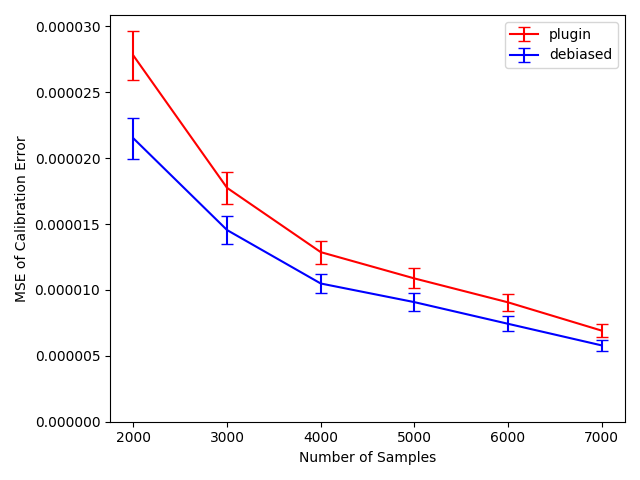
\includegraphics[width=\textwidth]{images/cifar_scaling_ece_curve_15.png}
         \caption{$B = 15$
         }
     \end{subfigure}
     \hfill
     \begin{subfigure}[b]{0.45\textwidth}
         \centering
         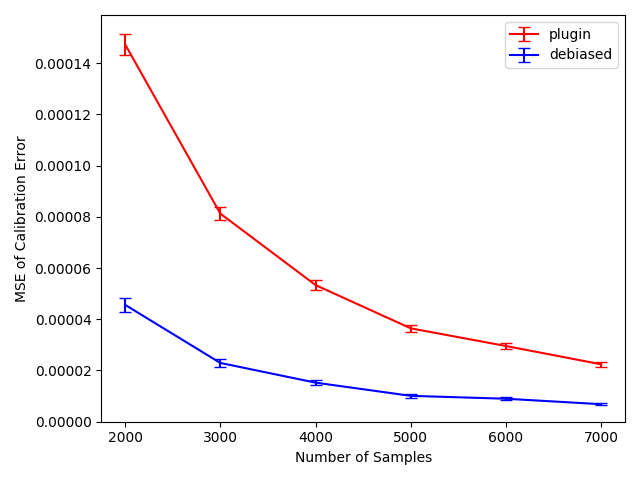
\includegraphics[width=\textwidth]{images/cifar_scaling_ece_curve_100.png}
         \caption{$B = 100$
         }
     \end{subfigure}
  \caption{
    Mean-squared errors of plugin and debiased estimators on a recalibrated VGG16 model on CIFAR-10 with $90\%$ confidence intervals (lower values better). The debiased estimator is closer to the ground truth, which corresponds to $0$ on the vertical axis, especially when $B$ is large or $n$ is small.
    Note that this is the MSE of the ECE estimates, not the MSE of the model in Figure~\ref{fig:nan2}.
}
  \label{fig:mse_estimators_cifar_ece_bins}
\end{figure}

For CIFAR-10 we use the same protocol except we split the validation set of size 10,000 into two sets $\calset{}$ and $\verifset{}$ of sizes 3,000 and 7,000 respectively. Figure~\ref{fig:mse_estimators} shows that the debiased estimates are much closer to the ground truth than the plugin estimates in this case as well.


\subsection{Additional experiments for estimating calibration error}

In Section~\ref{sec:verifying_calibration} we ran an experiment on CIFAR-10 to show that the debiased estimator gives estimates closer to the true calubration error than the plugin estimator. To give more insight into this, Figure~\ref{fig:histograms_estimators_bins} shows a histogram of the absolute difference between the estimates and ground truth for the plugin and debiased estimator, over the 1,000 resamples, when we use $B = 10$ or $B = 100$ bins. For $B = 10$ bins it is not completely clear which estimator is doing better but the debiased estimator avoids very bad estimates. However, when $B = 100$, the debiased estimator produces estimates much closer to the ground truth ($0$ on the x-axis).

\begin{figure}
  \centering
  \centering
     \begin{subfigure}[b]{0.45\textwidth}
         \centering
         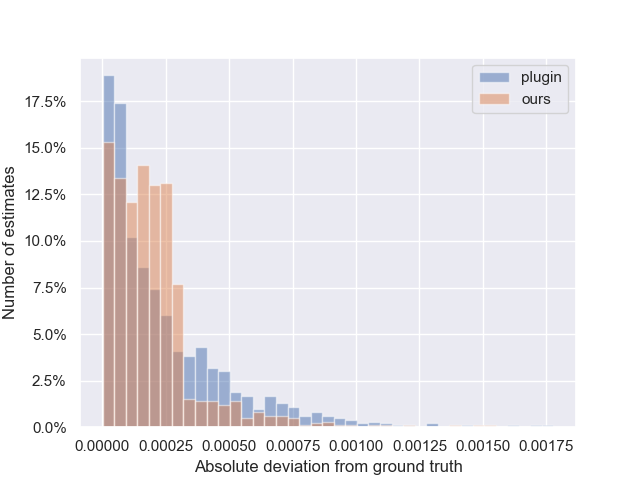
\includegraphics[width=\textwidth]{histogram_estimators_10_bins.png}
         \caption{$B = 10$ bins}
     \end{subfigure}
     \hfill
     \begin{subfigure}[b]{0.45\textwidth}
         \centering
         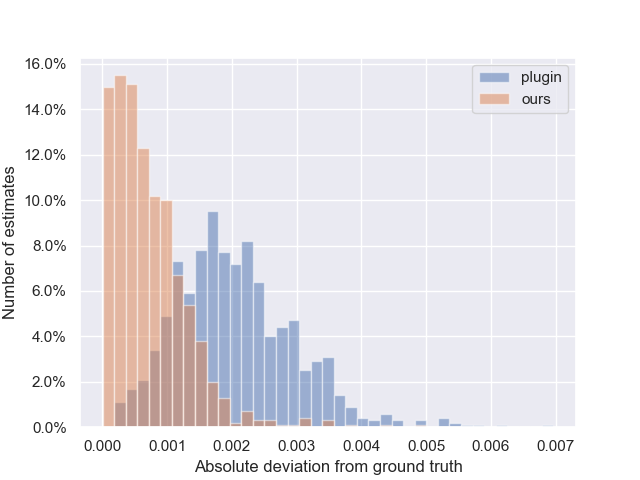
\includegraphics[width=\textwidth]{histogram_estimates_100_bins.png}
         \caption{$B = 100$ bins}
     \end{subfigure}
  \caption{Histograms of the absolute value of the difference between estimated and ground truth squared calibration errors ($0$ on the x-axis). For $B = 10$ bins, the results are mixed but we avoid very bad estimates. For $B=100$ our estimates are much closer to ground truth.\tnote{same comments as before}}
  \label{fig:histograms_estimators_bins}
\end{figure}

We also show histograms for the ECE experiments in Appendix~\ref{sec:debiasing_ece_experiments}, in Figure~\ref{fig:histograms_estimators_ece_imagenet_bins} for ImageNet and Figure~\ref{fig:histograms_estimators_ece_cifar_10_bins} for CIFAR-10. These histograms show that the proposed debiased estimator produces estimates much closer to the ground truth than the plugin estimator.

\begin{figure}
  \centering
  \centering
     \begin{subfigure}[b]{0.45\textwidth}
         \centering
         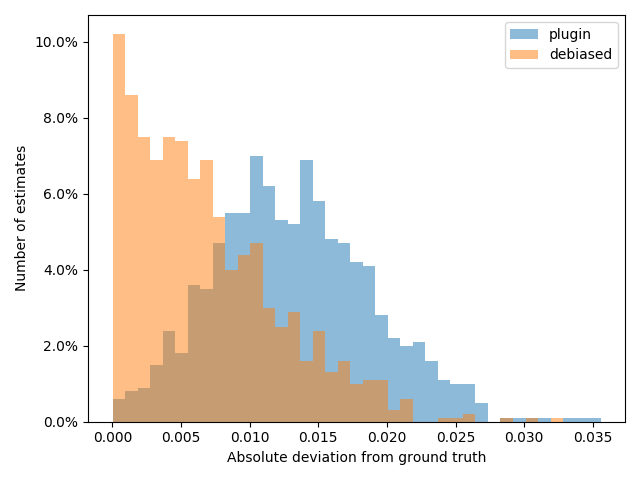
\includegraphics[width=\textwidth]{imnet_scaling_ece_histogram_15.png}
         \caption{$B = 15$ bins}
     \end{subfigure}
     \hfill
     \begin{subfigure}[b]{0.45\textwidth}
         \centering
         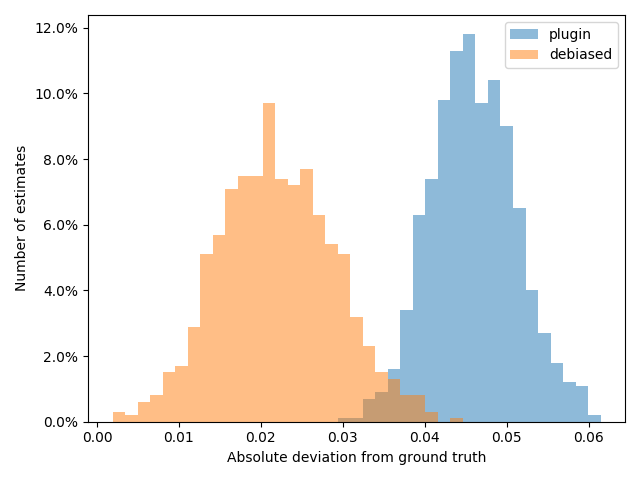
\includegraphics[width=\textwidth]{imnet_scaling_ece_histogram_100.png}
         \caption{$B = 100$ bins}
     \end{subfigure}
  \caption{Histograms of the absolute value of the difference between estimated and ground truth ECE ($0$ on the x-axis) on ImageNet.}
  \label{fig:histograms_estimators_ece_imagenet_bins}
\end{figure}

\begin{figure}
  \centering
  \centering
     \begin{subfigure}[b]{0.45\textwidth}
         \centering
         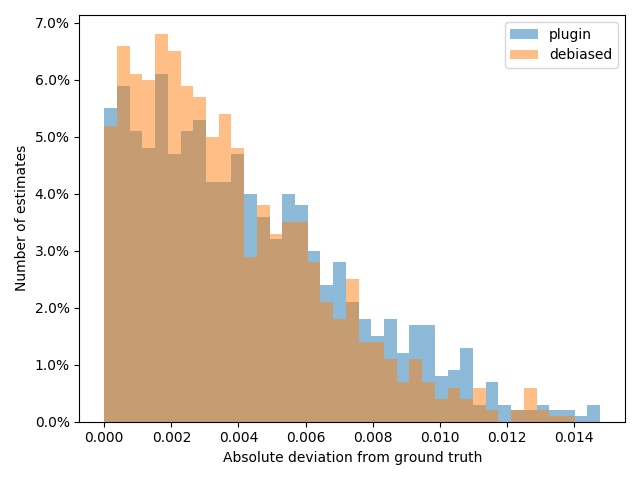
\includegraphics[width=\textwidth]{cifar_scaling_ece_histogram_15.png}
         \caption{$B = 15$ bins}
     \end{subfigure}
     \hfill
     \begin{subfigure}[b]{0.45\textwidth}
         \centering
         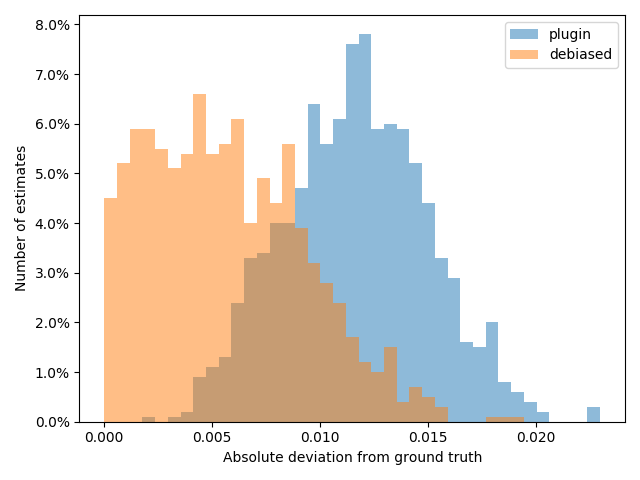
\includegraphics[width=\textwidth]{cifar_scaling_ece_histogram_100.png}
         \caption{$B = 100$ bins}
     \end{subfigure}
  \caption{Histograms of the absolute value of the difference between estimated and ground truth ECE ($0$ on the x-axis) on CIFAR-10.}
  \label{fig:histograms_estimators_ece_cifar_10_bins}
\end{figure}

We also ran a marginal multiclass calibration experiment on CIFAR-10 to show that our estimator allows us to select models with a lower mean-squared error subject to a given calibration constraint. In this case we split the validation set into $\calset{}$ and $\verifset{}$ of size 6000 and 4000 respectively, and recalibrated a trained model on $\calset{}$. On $\verifset{}$, we estimate the calibration error using the plugin and debiased estimators and use 100 Bootstrap resamples to compute a 90\% upper confidence bound on the estimate (from the variance of the Bootstrap samples). We compute the mean-squared error and the upper bounds on the calibration error for $B = 10, 15, \dots, 100$ and show the Pareto curve in Figure~\ref{fig:mse_vs_ce_estimator}. Figure~\ref{fig:mse_vs_ce_estimator} shows that for any desired calibration error, the debiased estimator enables us to pick out models with a better mean-squared error. For example, if we want a model with calibration error less than $1.5\%$, the debiased estimator tells us we can confidently use 100 bins, while relying on the plugin estimator only lets us use 15 bins and incurs a 13\% higher mean-squared error.

% Note that in our theoretical results in Section~\ref{sec:verifying_calibration}, we focused on hypothesis testing, using the estimator to test whether a model has calibration error $\leq \epsilon$ or not. However, the 

% \pl{say explicitly that we never say 'not calibrated'; there's a disconnect between the theory, which requires $r$ and $\epsilon$ and what we're doing here}



\begin{figure}
  \centering
  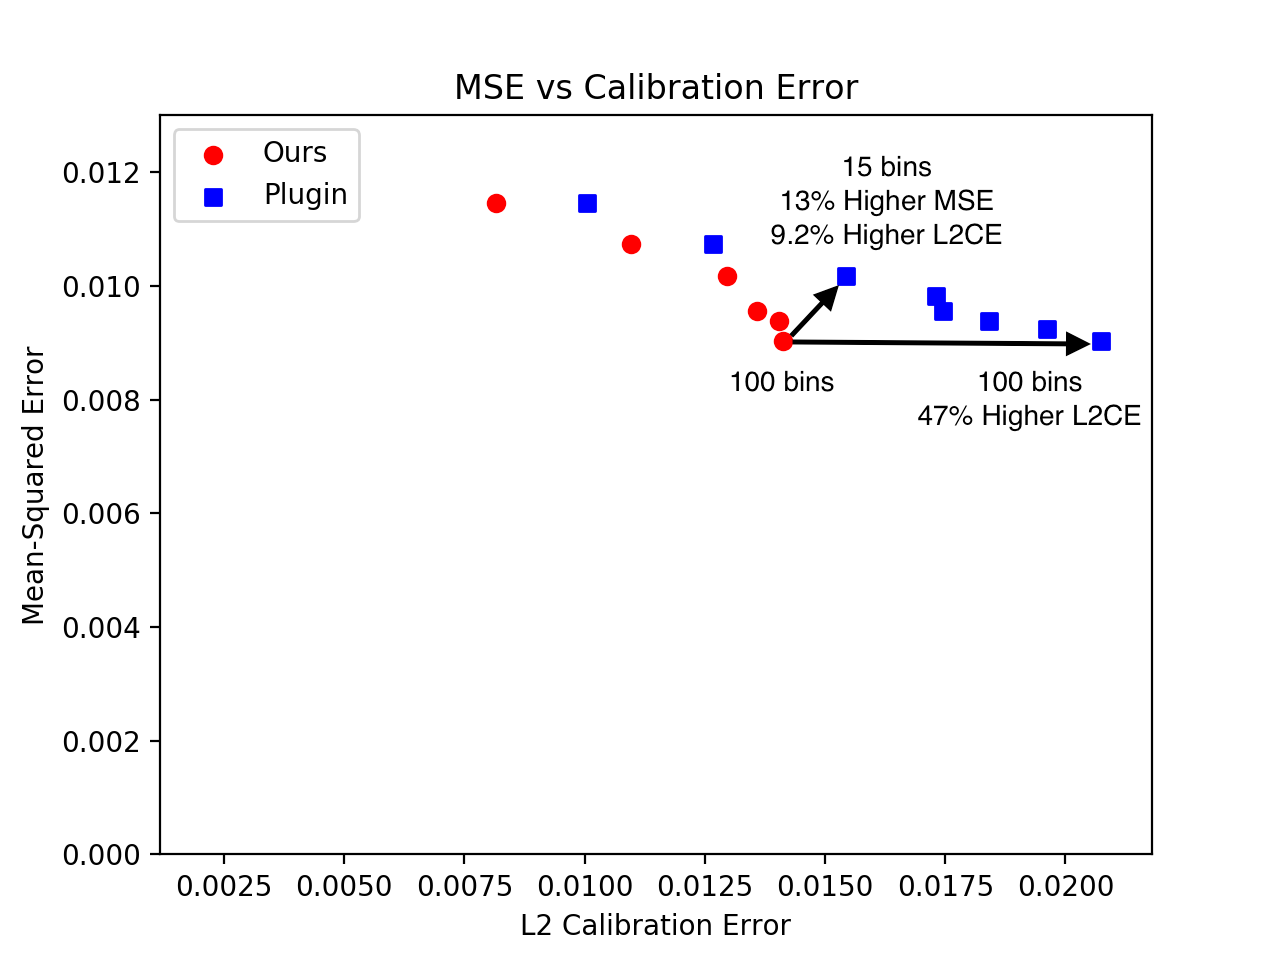
\includegraphics[width=0.9\textwidth]{mse_vs_verified_error_plugin_vs_ours.png}
  \caption{Plot of mean-squared error against 90\% upper bounds on the calibration error computed by the debiased estimator and the plugin estimator, when we vary the number of bins $B$. For a given calibration error, our estimator enables us to choose models with a better mean-squared error. If we want a model with calibration error less than 0.015, the debiased estimator tells us we can confidently use 100 bins, while relying on the plugin estimator only lets us use 15 bins and incurs a 13\% higher mean-squared error.}
  \label{fig:mse_vs_ce_estimator}
\end{figure}

